\section{Convolutional Nerual Networks}
\label{sec:cnn_theory}
This section describes what a \gls{cnn} is and what structure is used for creating the iris recognition \gls{cnn}. The section is based mainly on \cite{Karpathy2016a} and \cite{Nielsen2015}.

\subsection{Convolution}
A \gls{cnn} is a type of Nerual Network that is especially good for image recognition. Instead of the input being fully connected it operates by using a kernel instead. A kernel can be seen as a small window which moves through the input image. It performs an operation known as a convolution where the coefficients, also known as weights, of the kernel are multiplied with the pixel it is covering and summing the value. A 1D example of this is shown in \autoref{fig:kernel_convolution_example} where a kernel of size three with weights $\begin{bmatrix} 1 & 0 & -1 \end{bmatrix}$ is convolved through bottom rows which produces the top rows. Two other concepts are also shown in the example; stride and zero padding. Stride is the amount the kernel moves each time. The left example has a stride of one and the right example has a stride of two. Zero padding is when pixels with value $0$ are added at the edge of the image. This is done to ensure that the convolution can actually be made on all pixels, otherwise only two convolutions would be possible in the example with a stride of two. It also has the benefit of keeping the dimensions of the input image and output image the same when the stride is one, as convolution otherwise shrinks the image. 

\begin{figure}[h]
	\centering
	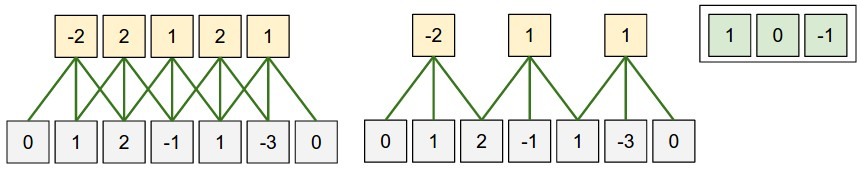
\includegraphics[width=0.90\textwidth]{kernel_convolution_example.jpeg}
	\caption{Example of a kernel in a \gls{cnn} \citep{Karpathy2016a}}
	\label{fig:kernel_convolution_example}
\end{figure}

The output of the convolution creates a new image. This image becomes the input of an activation function. An activation can be thought of as how much should the neuron fire, e.g how active is it. A common activation function for \gls{cnn} is the \gls{relu}, shown in \autoref{eq:ReluFunction}, which gives an output of $x$ if the $x$ is positive and 0 otherwise. This activation function has proved to be consistently better and faster for deep neural networks than the previously popular sigmoid activation function.

\begin{equation}
\label{eq:ReluFunction}
f(x) = max(0,x)
\end{equation}

\subsection{Activation Function and Feature Maps}
The output of the convolution is the hidden layer and is called a feature map. An example is shown in \autoref{fig:cnn_kernal_illustration}, where a kernel of $5\times5$ with stride one is used on a input image of $28\times28$ to produce a feature map of $24\times24$. The dimensions can be calculated by using \autoref{eq:feature_map_size}  where $W_2$ is the width of the feature map, $W_1$ is the width of the input image, $F$ is the size of the kernel, $P$ is the amount of padding, and $S$ is the stride.  

\begin{equation}
\label{eq:feature_map_size}
W_2 = \frac{(W_1-F+2P)}{S} +1
\end{equation}

The weights of the kernel is what is being learned by the network. The kernel has what is known as shared weights and biases, as it is the same weights that convolve through the whole image. This is shown in \autoref{eq:shared_weights}, which is how a single neuron of the feature map in \autoref{fig:cnn_kernal_illustration} is computed. $\sigma$ is an activation function, $b$ is the shared bias,  $w$ are the weights of the kernel with $(l,m)$ being their position and $a$ is the input pixel at the position given by the coordinates $(j,k)$.

\begin{equation}
\label{eq:shared_weights}
\sigma(b+\sum\limits_{l=0}^L \sum\limits_{m=0}^M w_{l,m}*a_{j+l,k+m})
\end{equation}


In other words the kernel learns to detect a feature that can be found in the image, e.g. straight lines. As a single feature is not enough for recognition, multiple kernels are used to make multiple feature maps. These new feature maps become the input of another convolution layer that can learn higher level features, e.g. combining the vertical and horizontal features to create a kernel that detects edges. Each convolution adds a new level of abstraction.

\begin{figure}[h]
\centering
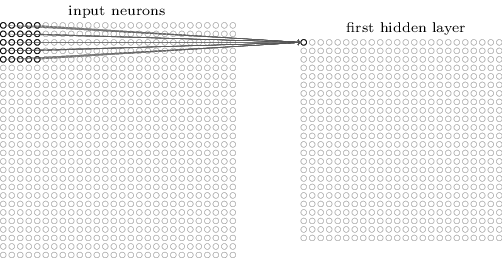
\includegraphics[width=0.90\textwidth]{cnn_kernal_illustration.png}
\caption{Example of a kernel in a \gls{cnn} \citep{Nielsen2015}}
\label{fig:cnn_kernal_illustration}
\end{figure}

\subsection{Pooling}
Pooling is an operation often added after a convolutional layer. Like a convolution, a small window moves through the image, except it does not convolve but simply looks at the pixels in its current location and outputs a single pixel depending of the type of pooling used. Maxpooling is a common type of pooling used in \gls{cnn}s. An example of maxpooling with a window of size $2\times2$ and stride two is shown in \autoref{fig:maxpool_example}. This has the benefit of downscaling the spatial size of the image for faster computation and reducing overfitting.

\begin{figure}[H]
\centering
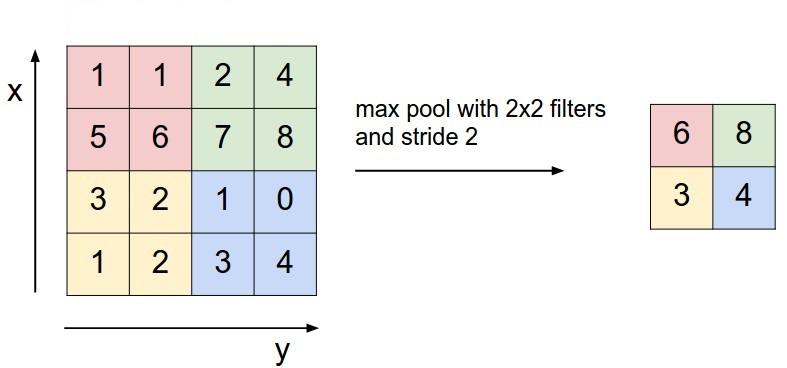
\includegraphics[width=0.90\textwidth]{maxpool_example.jpeg}
\caption{Example of maxpooling with size $2x2$ and stride 2 \citep{Karpathy2016a}}
\label{fig:maxpool_example}
\end{figure}

\subsection{Classification}
To use the features extracted from the convolutional layer one or more \gls{fc} layers are added at the end of a network. In an \gls{fc} layer all the neurons from the previous layer are connected to all of the neurons in current layer. This relationship is shown in \autoref{eq:fully_connected_layer}. The output of a single neuron is the sum of all the previous weights $w_i$ and their bias $b$ put through some activation function $f$.

\begin{equation}
\label{eq:fully_connected_layer}
f\left(\sum_{i}w_{i}x_{i}+b\right)
\end{equation}

To classify $N$ number of classes the last \gls{fc} layer usually has the same amount of neurons as classes. A common activation function for multi class categorisation is the softmax function. It is a normalised exponential function that calculates the probability of each class over all possible classes. The outputs are in a range of $0 - 1$ and the sum of all class probabilities is 1. The function is described in \autoref{eq:softmax_activation_function} where $Z$ is a vector of weights from the previous layer, $j$ is the output class and $K$ is the total amount of classes.

\begin{equation}
\label{eq:softmax_activation_function}
\sigma(Z)_{j} = \frac{e^{Z_j}}{\sum_{k=1}^{K}e^{Z_k}}
\end{equation}

A common loss function that is used to optimise the softmax function is a cross-entropy loss function. Cross-entropy is defined as in \autoref{eq:cross_entropy_function} where $q$ is the estimated distribution and $p$ is the actual distribution. In other words it's a measurement of how far the estimated classes are from the true classes.
\begin{equation}
\label{eq:cross_entropy_function}
H(p,q) = -\sum_{x}p(x)log(q(x))
\end{equation}
The estimated classes are given by the softmax function, in other words $q = \sigma(Z)_{j} $. The loss function that is optimised is then \autoref{eq:cross_entropy_loss_function}.
\begin{equation}
\label{eq:cross_entropy_loss_function}
J(\theta) = -\frac{1}{m}\left[ \sum_{i=1}^{m}\sum_{j=1}^{K} 1\{y_i=j\}  log\left( \frac{e^{\theta_j}}{\sum_{k=1}^{K}e^{\theta_k}} \right)\right] + \frac{\lambda}{2} \sum_{i=1}^{K} \sum_{j=0}^{n} \theta_{ij}^{2}
\end{equation}
Where $\theta$ is the weights that are randomly set and are learned through back propagation. $K$ is the number of classes and $n$ is the number of labelled training samples. $y_i$ is the label and $1\{\cdot\}$ is a function that is 1 when the input is true and 0 when it is not. The second term is weight decay regularization term that reduces the magnitudes of weights and prevents it from overfitting.


\subsection{Network Construction}
To construct and train the networks, Keras is used with Tensorflow as a backend. Keras is an API written in Python, able to run on three different backends. With a high level of modularity by having separate models added on top of each other construction and overview of a network is simplified. By using Tensorflow with Keras it is possible to utilise a Conda compatible \gls{gpu}, which decreases the training time compared to the training time when using only a \gls{cpu}. Keras has several example programs from which inspiration and techniques can be gathered but also contains well known specific models to implement and configure in a new network. This includes the VGG16 network including weights trained on the ImageNet database with 2000 different classes.



%$l$ denotes the current layer and $l-1$ is the previous layer. $y^{l}(j)$ is the output of neuron $j$ at \gls{fc} layer $l$. It is a linear combination of the weights and biases from the previous layer put into an activation function $f^l$. $ y^{l-1}(i).w^{l}(i,j)$ is the weight from neuron $j$ in the previous layer $l-1$ to the neuron $j$ in current layer $l$
%This creates many more weights to train compared to the weights of a kernel. \todo{diskuter om vi måske skulle bruge subscript i den her ligning, selvom de ikke gør det i artiklen}
%\begin{eqnarray}
%\label{eq:fully_connected_layer}
%y^{l}(j)=f^{l}(\sum\limits_{i=1}^{N^{l-1}} y^{l-1}(i).w^{l}(i,j)+b^{l}(j)(3))
%\end{eqnarray}

\section{Iris Recognition}
\label{sec:cnn_iris_rec}
The structure for the iris \gls{cnn} is based on work done by \cite{Al-Waisy2017}. They made a structure named IrisConvNet that uses a segmented and normalised iris image, described in \autoref{sec:irisnorm} to classify. For training they tried three iris databases; SDUMLA-HMT, CASIA-Iris-V3 and IITD. The \gls{cnn}s were only trained and tested on one database at a time.  The normalised images were originally $256\times70$ and $256\times135$. The images were resized to be squares with the size of the shortest dimension. To produce more samples data augmentation was performed. Five $64\times64$ images were generated by cropping the rescaled image corresponding to images from the four corners and a centre image. These images were also flipped horizontally, totalling in ten images augmented from a single image. Different amounts of feature maps were tested to get the best classifier. The general structure was the same. They tried \gls{cnn}s with three to five convolutional layers with $2\times2$ maxpooling in between. The first kernel was $3\times3$ and the rest were $5\times5$. At the end there are two \gls{fc} layers and a prediction layer. The input sizes are $64\times64$ or $128\times128$. They varied the amount of feature maps with the first layer having six feature maps and the following layers having a gradually increasing number of feature maps. The best performing configuration for the $64\times64$ images achieved between 99.62\% and 100\% accuracy between the databases. It had four convolutional layers with respectively 6, 32, 64, and 256 feature maps. For input images of size $128\times128$ the best configuration achieved between 99.41\% and 100\% accuracy. It had five layers with respectively 6, 16, 32, 64, and 256 feature maps.

\subsection{Parameters and Settings}
\cite{Al-Waisy2017} had various parameters and settings for their network, which are listed for ease of replication. They deemed 500 epochs to be an appropriate amount of training before it started overfitting. They used AdaGrad optimiser with a learning rate of $10^{-2}$ with a weight decay of 0.0005. The \gls{relu} activation function was used for convolutions and the two \gls{fc} layers, while the classifying layer used softmax and cross-entropy as the loss function. They also had a dropout layer of 0.5 in between the two \gls{fc} layers. This means that during each iteration each node has a 50\% probability of being ignored, which helps prevent interdependencies among the nodes to appear and reduces overfitting. Zero padding of one pixel is added on the input image which changes its dimensions from $64\times64$ to $66\times66$. The number of neurons in the \gls{fc} layers were not specified except for the classifying layer having the same amount of neurons as classes. 

\subsection{Project Solution}

As previously stated the solution for the network is heavily based on the structure used by \cite{Al-Waisy2017} but with alterations and applied on the Warsaw-BioBase database. An overview of the design is shown in \autoref{fig:iris_cnn}. The learning rate is set to $10^{-3}$ as $10^{-2}$ turned out to be too big. The original normalised iris is $64\times 512$ so it is resized to $64\times64$. The data augmented images then becomes $58\times58$. The two \gls{fc} layers are set to 1024 as they have not been specified by \cite{Al-Waisy2017}. The same optimiser and hyper parameters are used.

\begin{figure}[H]
	\centering
	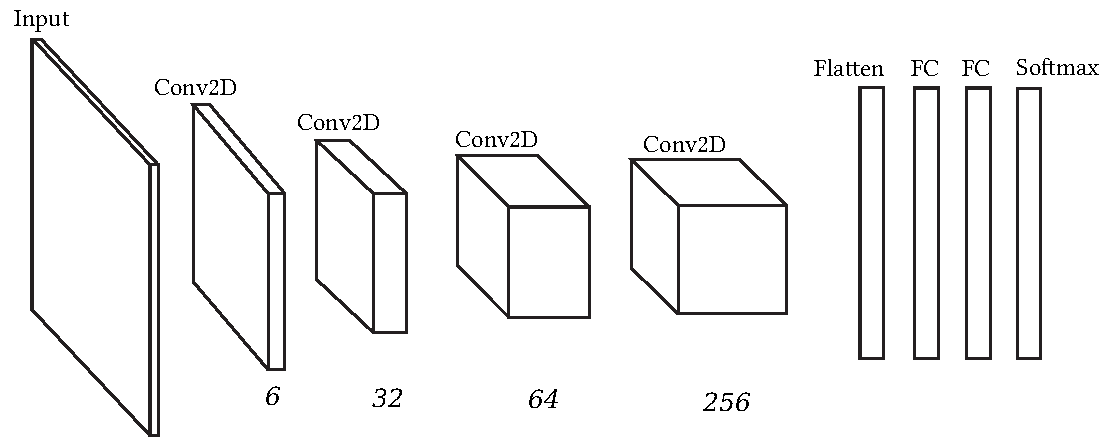
\includegraphics[width=0.8\textwidth]{network_iris}
	\caption{Overview of the iris recognition network design}
	\label{fig:iris_cnn}
\end{figure}

A more detailed description of the network is shown in \autoref{tab:iris_cnn}.

\begin{table}[H]
	\centering
	\caption{Detailed description of network design and settings}
	\label{tab:iris_cnn}
	\begin{tabular}{lrrrr}
		\textbf{Layer Type}   & \textbf{Feature Map Size}  & \textbf{Kernel/Pool Size} & \textbf{Activation} & \textbf{Other} \\ \hline
		Conv2D       & $6$               & $3\times3$       & ReLU       &       \\
		\rowcolor{lightGrey} 
		MaxPooling2D &                   & $2\times2$       &            &       \\
		Conv2D       & $32$              & $5\times5$       & ReLU       &       \\
		\rowcolor{lightGrey} 
		MaxPooling2D &                   & $2\times2$       &            &       \\
		Conv2D       & $64$              & $5\times5$       & ReLU       &       \\
		\rowcolor{lightGrey} 
		MaxPooling2D &                   & $2\times2$       &            &       \\
		Conv2D       & $256$             & $5\times5$       & ReLU       &       \\
		\rowcolor{lightGrey} 
		Flatten      &                   &                  &            &       \\
		Dense        & 1024              &                  & ReLU           &       \\
		\rowcolor{lightGrey} 
		Dropout      &                   &                  &            & $0.5$ \\
		Dense        & 1024              &                  & ReLU           &       \\
		\rowcolor{lightGrey} 
		Dropout      &                   &                  &            & $0.5$ \\
		Dense        & Amount of Classes &                  & Softmax   &      
	\end{tabular}
\end{table}

To train and evaluate the model, the dataset is split into three sets; training, validation and testing. The model is trained on the training set while being evaluated on the validation set. The model parameters are then adjusted on the basis of the validation set. Finally it is evaluated on the testing set. The split is 70\%, 15\%, 15\%. The accuracy is defined simply by:
\begin{equation}
\text{Accuracy} = \frac{\text{Correct Categorisation}}{\text{Total number}}\cdot100 
\end{equation}
The results achieved with this network is an accuracy of $99.7\%$. This is achieved with a batch size of $128$ and $200$ epochs. In \autoref{fig:iris_graphs} the accuracy and loss progression is shown.

\begin{figure}[H]
	\centering
	\begin{subfigure}{0.48\textwidth}
		\centering
		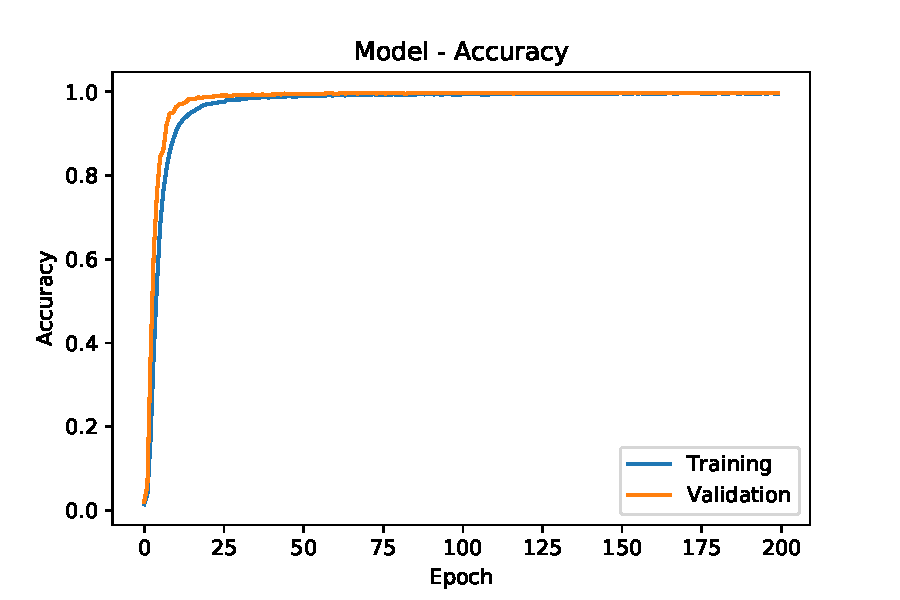
\includegraphics[width=\textwidth]{iris_cnn_acc}
		\caption{\gls{cnn} accuracy progression through epochs}
		\label{fig:iris_cnn_acc}
	\end{subfigure}
	\begin{subfigure}{0.48\textwidth}
		\centering
		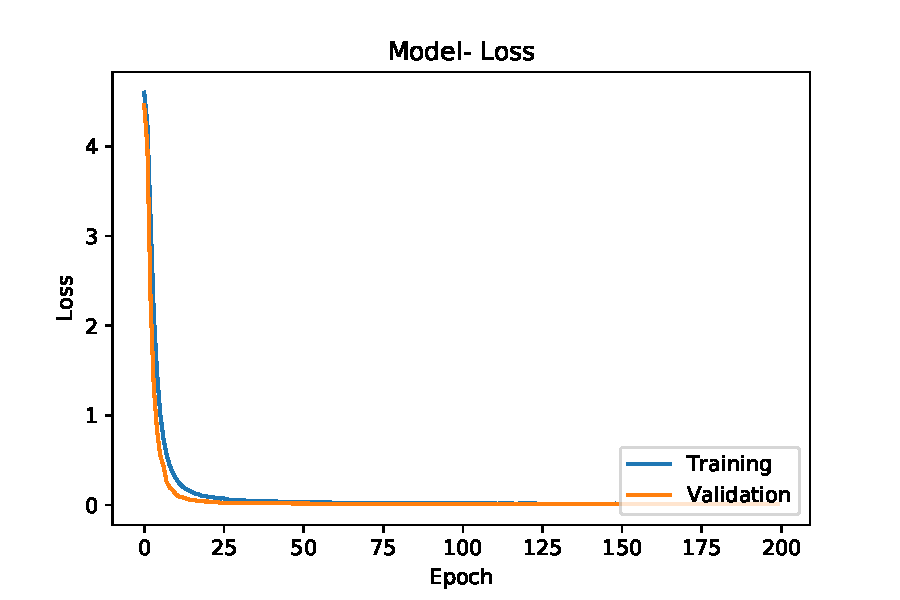
\includegraphics[width=\textwidth]{iris_cnn_loss}
		\caption{\gls{cnn} loss progression through epochs}
		\label{fig:iris_cnn_loss}
	\end{subfigure}
	\caption{Accuracy and loss progression for the iris recognition \gls{cnn}.}
	\label{fig:iris_graphs}
\end{figure}
\todo[inline]{Add bridge to face recognition - why are we going there now?}

\section{Face Recognition}
To make a face recognition \gls{cnn} an already well known model is used. The network is based on the VGG16 model, including the weights pre-trained on the ImageNet database with 2000 classes. The model is split into five blocks. The input size of the images are $64\times64\times3$ and are from the \gls{lfw} database. The network is made and well known for image classification, and with the pre-trained weights from ImageNet, it is a suitable solution for face recognition \citep{Simonyan2015}.
An overview of the network is shown in \autoref{fig:vgg16} and a more detailed setup description is shown in \autoref{tab:vgg16}. The network gets an accuracy of $99.35\%$ on the \gls{lfw} database. \autoref{fig:vgg_graphs} shows the accuracy and loss progression.

\begin{figure}[H]
	\centering
	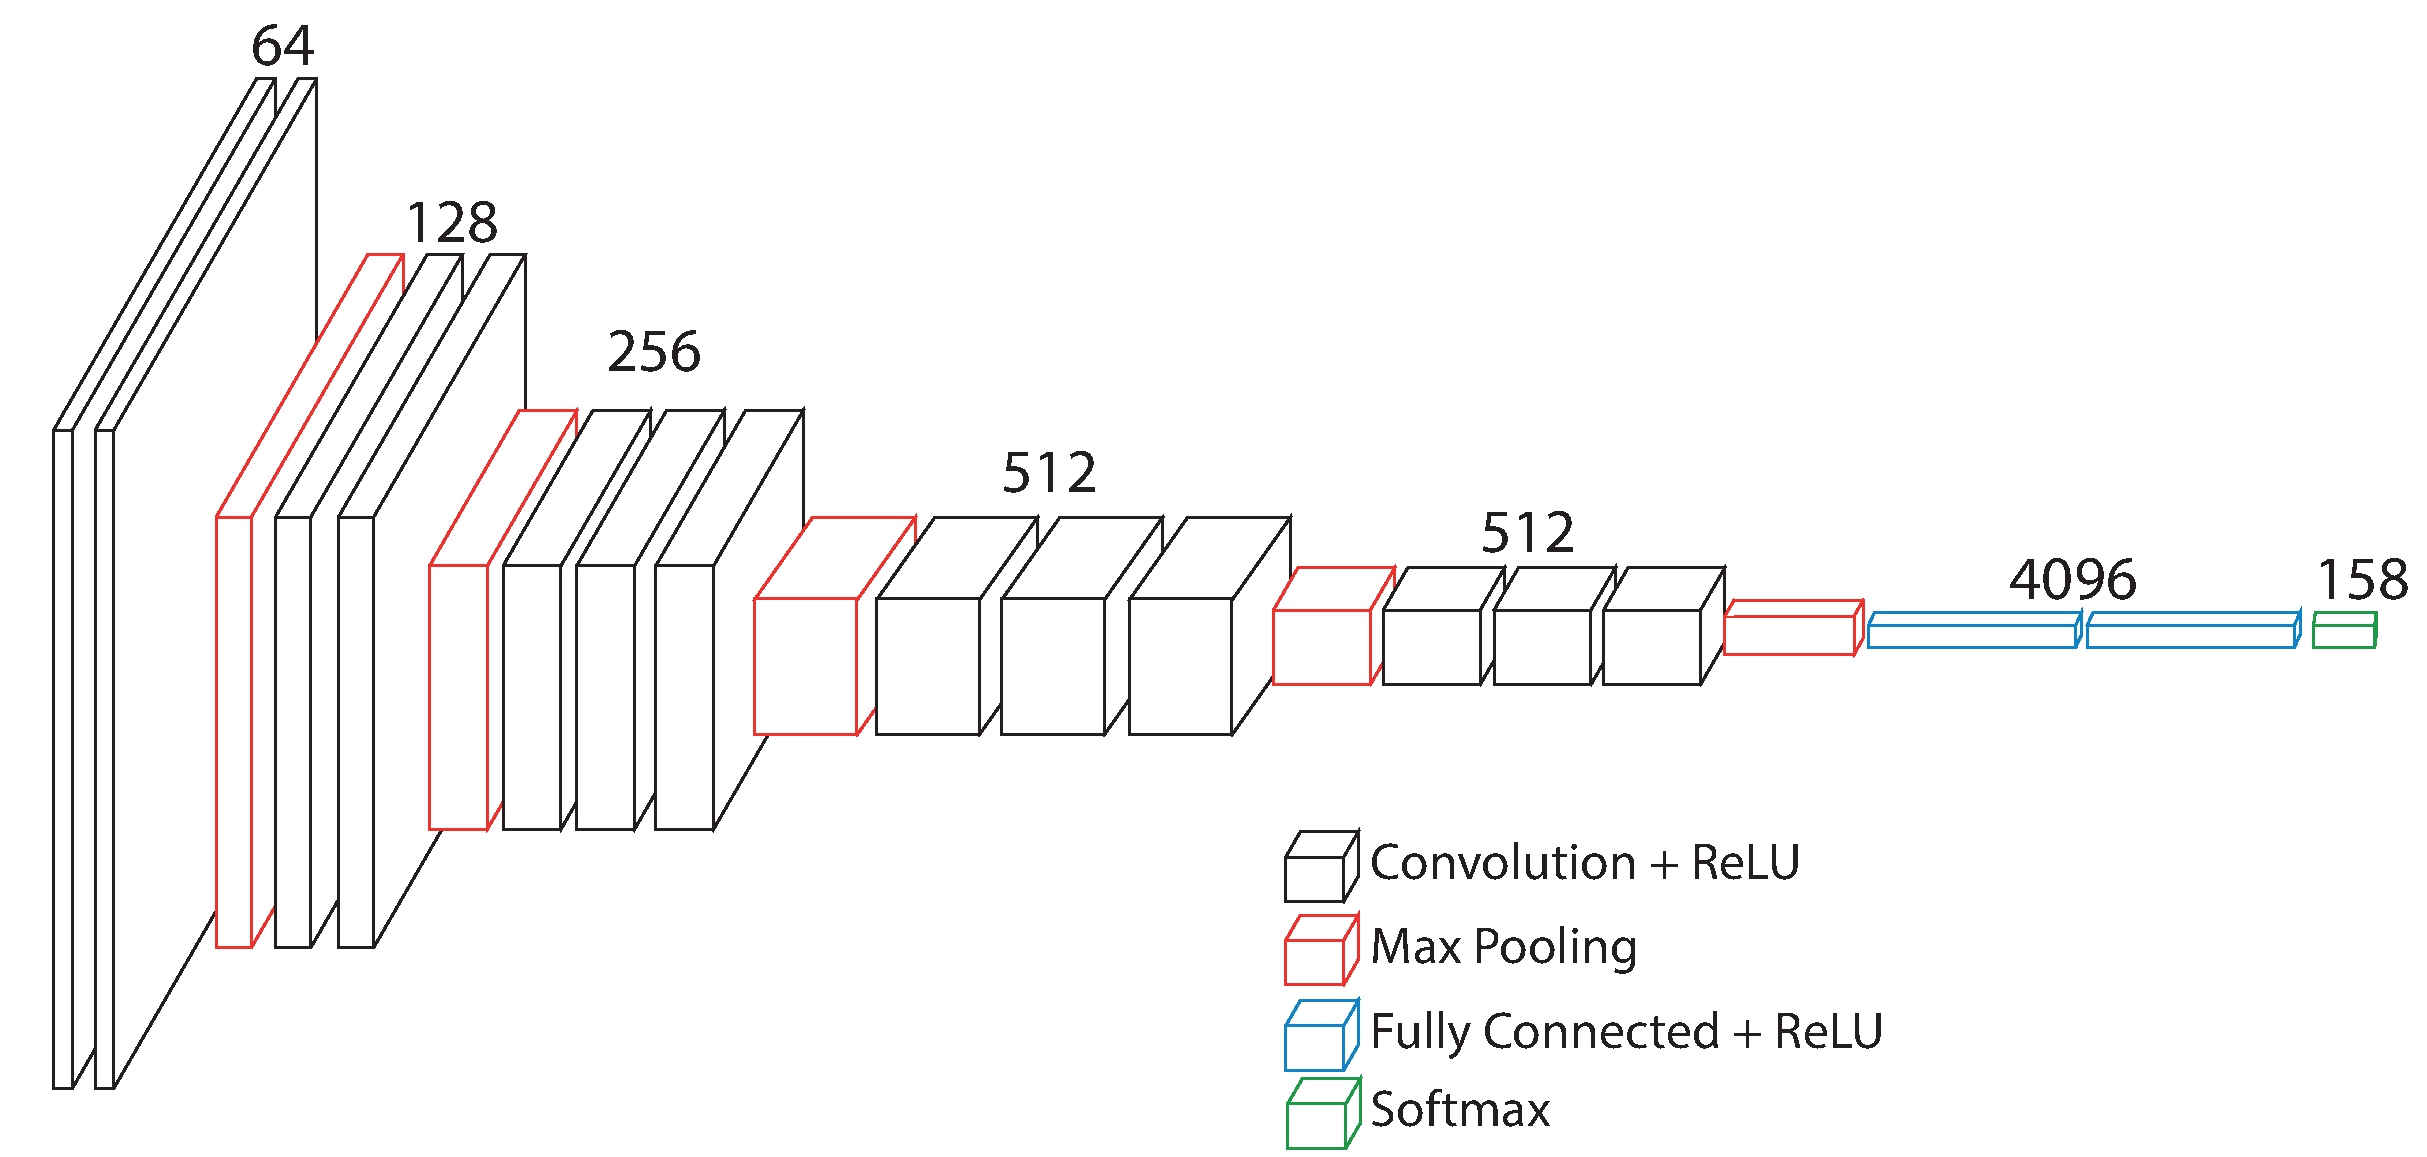
\includegraphics[width=\textwidth]{vgg16_overview}
	\caption{Overview of the VGG16 \gls{cnn} used for face recognition. Only the depth of the layers is known and noted. The input is excluded from the figure.}
	\label{fig:vgg16}
\end{figure}

\begin{table}[H]
	\centering
	\caption{Detailed description of VGG16 design. The input is $64\times64\times3$ images.}
	\label{tab:vgg16}
	\begin{tabular}{lrrrr}
		\textbf{Layer Type}     & \textbf{Feature Map Size} & \textbf{Kernel/Pool Size} & \textbf{Activation} & \textbf{Other} \\ \hline
		\textbf{Block 1}        &                           &                           &                     &                \\
		\rowcolor{lightGrey}  
		Conv2D                  & $64$                      & $3\times3$                & ReLU                &                \\
		Conv2D                  & $64$                      & $3\times3$                & ReLU                &                \\
		\rowcolor{lightGrey} 
		MaxPooling2D            &                           & $2\times2$                &                     &                \\
		\textbf{Block 2}        &                           &                           &                     &                \\
		\rowcolor{lightGrey}  
		Conv2D                  & $128$                     & $3\times3$                & ReLU                &                \\
		Conv2D                  & $128$                     & $3\times3$                & ReLU                &                \\
		\rowcolor{lightGrey}  
		MaxPooling2D            &                       &    $2\times2$             & ReLU                &                \\
		\textbf{Block 3}        &                           &                           &                     &                \\
		\rowcolor{lightGrey}  
		Conv2D                  & $256$                     & $3\times3$                & ReLU                &                \\
		Conv2D                  & $256$                     & $3\times3$                & ReLU                &                \\
		\rowcolor[HTML]{EFEFEF} 
		Conv2D                  & $256$                     & $3\times3$                & ReLU                &                \\
		MaxPooling2D            &               &          $2\times2$                  &                     &                \\
		\textbf{Block 4}        &                           &                           &                     &                \\
		\rowcolor{lightGrey}  
		Conv2D                  & $512$                     & $3\times3$                & ReLU                &                \\
		Conv2D                  & $512$                     & $3\times3$                & ReLU                &                \\
		\rowcolor{lightGrey}  
		Conv2D                  & $512$                     & $3\times3$                & ReLU                &                \\
		MaxPooling2D            &             &          $2\times2$                  &                     &                \\
		\textbf{Block 5}        &                           &                           &                     &                \\
		\rowcolor{lightGrey}  
		Conv2D                  & $512$                     & $3\times3$                & ReLU                &                \\
		Conv2D                  & $512$                     & $3\times3$                & ReLU                &                \\
		\rowcolor{lightGrey}  
		Conv2D                  & $512$                     & $3\times3$                & ReLU                &                \\
		MaxPooling2D            &               &        $2\times2$        & ReLU                &                \\
		\textbf{Classification} &                           &                           &                     &                \\
		\rowcolor{lightGrey}  
		Flatten                 &                           &                           &                     &                \\
		Dense                   & $4096$                    &                           & ReLU                &                \\
		\rowcolor{lightGrey}  
		Dropout                 &                           &                           &                     & $0.5$          \\
		Dense                   & $4096$                    &                           & ReLU                &                \\
		\rowcolor{lightGrey} 
		Dropout                 &                           &                           &                     & $0.5$          \\
		Dense                   & Amount of Classes         &                           & Softmax             &               
	\end{tabular}
\end{table}

\begin{figure}[H]
	\centering
	\begin{subfigure}{0.48\textwidth}
		\centering
		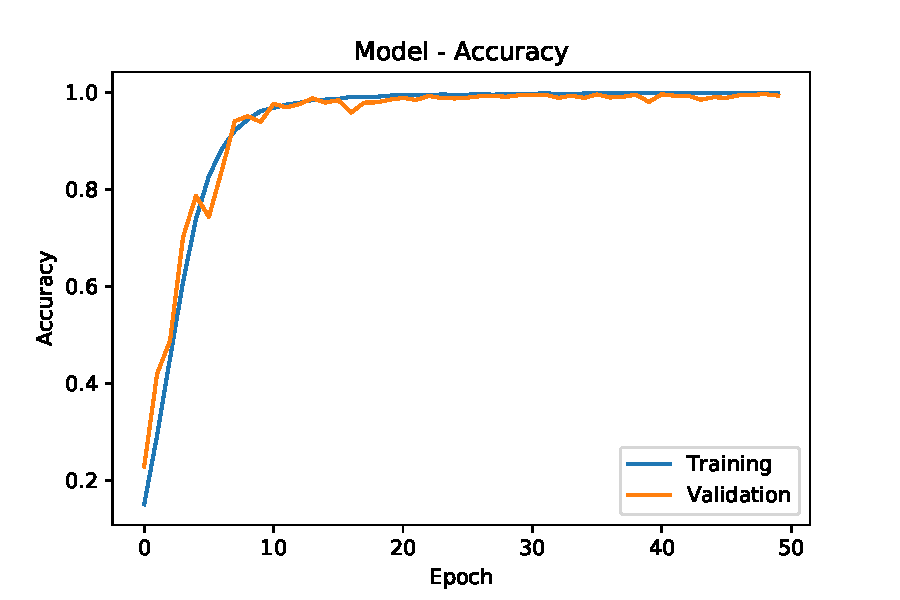
\includegraphics[width=\textwidth]{vgg16_acc}
		\caption{Face recognition \gls{cnn} accuracy progression through epochs}
		\label{fig:vgg16_acc}
	\end{subfigure}
	\begin{subfigure}{0.48\textwidth}
		\centering
		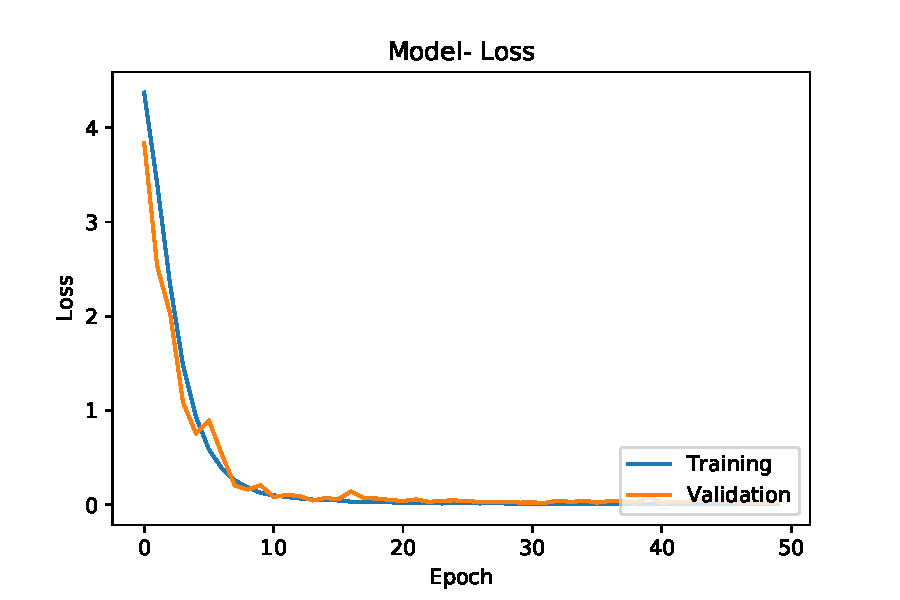
\includegraphics[width=\textwidth]{vgg16_loss}
		\caption{Face recognition \gls{cnn} loss progression through epochs}
		\label{fig:vgg16_loss}
	\end{subfigure}
	\caption{Accuracy and loss progression for the face recognition VGG16 \gls{cnn}.}
	\label{fig:vgg_graphs}
\end{figure}
